%========================================================================================
%  CAPITOLO 2 — PULSAR TIMING ARRAY
%  Obiettivo: spiegare cosa sono le pulsar, come si misurano i TOA e i residui, come
%  un'onda gravitazionale modifica i residui, perché serve un ARRAY (Hellings-Downs) e
%  quali sono i risultati attuali. Chiudere motivando il problema del rumore (-> cap. 3).
%  Lunghezza indicativa: 6-8 pagine.
%  Fonti principali: Taylor (2021) cap. 3, Shaifullah (2025) sez. 2-4 e 6, tesi di Irene cap. 2.
%========================================================================================

\chapter{Pulsar Timing Array} \label{chpt:PTA}
\sloppy

Un \textit{Pulsar Timing Array} (PTA) è un rivelatore di onde gravitazionali di dimensioni galattiche, costituito da un insieme di pulsar al millisecondo monitorate regolarmente con i radiotelescopi per decine di anni~\cite{FosterBacker1990}. L'idea, proposta già alla fine degli anni '70~\cite{Sazhin1978, Detweiler1979}, è usare le pulsar come orologi estremamente stabili: un'onda gravitazionale che attraversa lo spazio tra la Terra e una pulsar modifica il tempo di percorrenza degli impulsi radio, che arrivano leggermente in anticipo o in ritardo rispetto a quanto previsto. Confrontando questi ritardi in molte pulsar diverse è possibile distinguere il segnale gravitazionale, che è correlato tra le pulsar in un modo caratteristico, dalle numerose sorgenti di rumore proprie di ciascuna pulsar.

In questo capitolo descrivo le pulsar (Sezione~\ref{sec:pulsar}), la tecnica del \textit{pulsar timing} (Sezione~\ref{sec:timing}), la risposta dei tempi di arrivo a un'onda gravitazionale (Sezione~\ref{sec:risposta_GW}), il ruolo dell'array e della correlazione di Hellings e Downs (Sezione~\ref{sec:HD}) e infine lo stato attuale delle osservazioni (Sezione~\ref{sec:PTA_oggi}).

%%%%%%%%%%%%%%%%%%%%%%%%%%%%%%%%%%%%%%%%%%%%%%%%%%%%%%%%%%%%%%%%%%%%%%%%%%%%%%%%%%%%%%%%%%
\section{Pulsar e pulsar al millisecondo} \label{sec:pulsar}

Le pulsar sono stelle di neutroni in rapida rotazione e dotate di un campo magnetico molto intenso, scoperte nel 1967 da Jocelyn Bell e Antony Hewish~\cite{Hewish1968}. Una stella di neutroni è il residuo compatto del collasso del nucleo di una stella massiccia: ha una massa di circa $1.4\,\Msun$ concentrata in un raggio di $\sim 10$--$15$~km ed è sostenuta dalla pressione di degenerazione dei neutroni. Per conservazione del momento angolare e del flusso magnetico durante il collasso, la stella risultante ruota molto velocemente e ha campi magnetici superficiali tipicamente compresi tra $10^8$ e $10^{12}$~G~\cite{LorimerKramer2005}.

Le particelle cariche accelerate nella magnetosfera producono due fasci di radiazione radio lungo l'asse del dipolo magnetico. Poiché questo asse non è allineato con l'asse di rotazione, i fasci ruotano con la stella e, come la luce di un faro, vengono osservati dalla Terra come una sequenza di impulsi separati dal periodo di rotazione $P$ (\textit{modello a faro}, Figura~\ref{fig:faro}).

\begin{figure}[h!]
    \centering
    % \includegraphics[width=0.55\textwidth]{Figure/cap2/pulsar_faro.pdf}
    \fbox{\parbox{0.55\textwidth}{\centering\vspace{1.5cm}\TODO{figura: schema del modello a faro (asse di rotazione, asse magnetico, fasci radio)}\vspace{1.5cm}}}
    \caption{\footnotesize Schema del modello a faro di una pulsar.}
    \label{fig:faro}
\end{figure}

La maggior parte delle pulsar note ha periodi dell'ordine del secondo. Per i PTA sono però di interesse le \textit{pulsar al millisecondo} (\textit{millisecond pulsars}, MSP), la prima delle quali, PSR B1937+21, fu scoperta nel 1982~\cite{Backer1982}. Si tratta di pulsar vecchie che, trovandosi in un sistema binario, hanno accresciuto materia e momento angolare dalla stella compagna e sono state ``riaccelerate'' fino a periodi di pochi millisecondi. Le MSP hanno una rotazione straordinariamente regolare: il profilo dell'impulso mediato su molte rotazioni è stabile su tempi di decenni e il rallentamento della rotazione è molto lento. Per questo motivo si comportano come orologi la cui stabilità a lungo termine è paragonabile a quella degli orologi atomici~\cite{Taylor2021, LorimerKramer2005}.

La pulsar analizzata in questa tesi, PSR J1640+2224, è una MSP con periodo $P \simeq 3.16$~ms in orbita attorno a una nana bianca con un periodo orbitale di circa 175 giorni, ed è una delle 25 pulsar della seconda \textit{data release} dello \textit{European Pulsar Timing Array} (EPTA DR2)~\cite{EPTA2023_DR2data}. % TODO: verificare P e Pb su ATNF / paper EPTA DR2

%%%%%%%%%%%%%%%%%%%%%%%%%%%%%%%%%%%%%%%%%%%%%%%%%%%%%%%%%%%%%%%%%%%%%%%%%%%%%%%%%%%%%%%%%%
\section{La tecnica del pulsar timing} \label{sec:timing}

\subsection{Tempi di arrivo}

I singoli impulsi di una pulsar sono in genere troppo deboli per essere distinti dal rumore e hanno una forma variabile da una rotazione all'altra. Durante un'osservazione, che dura da qualche minuto a un'ora, si sommano quindi migliaia di impulsi ``ripiegando'' (\textit{folding}) il segnale sul periodo noto della pulsar: si ottiene così un profilo medio, molto più stabile e con un rapporto segnale/rumore elevato~\cite{Taylor2021}.

Prima del folding bisogna correggere l'effetto della dispersione nel mezzo interstellare ionizzato. L'indice di rifrazione del plasma dipende dalla frequenza, e gli impulsi osservati a frequenza radio $\nu$ più bassa arrivano più tardi, con un ritardo
\begin{equation}
    \Delta t_{\mathrm{DM}} \propto \frac{\mathrm{DM}}{\nu^2}\, , \qquad \mathrm{DM} = \int_0^L n_e\, \dd l \, ,
    \label{eq:ritardo_DM}
\end{equation}
dove la \textit{dispersion measure} (DM) è la densità di colonna degli elettroni liberi lungo la linea di vista. Questa dipendenza dalla frequenza radio (``cromatica'') tornerà nel Capitolo~\ref{chpt:rumore}, perché le variazioni temporali della DM sono una delle principali sorgenti di rumore.

Il profilo ottenuto viene confrontato con un profilo di riferimento (\textit{template}) ad alto rapporto segnale/rumore: lo sfasamento tra i due, sommato all'istante di inizio dell'osservazione, fornisce il \textit{tempo di arrivo} (\textit{time of arrival}, TOA) dell'impulso, con un'incertezza tipica dell'ordine di $0.1$--$1\ \upmu$s per le MSP migliori. Infine i TOA, misurati dall'osservatorio sulla Terra (che non è un sistema inerziale), vengono riportati al baricentro del Sistema Solare, tenendo conto del moto della Terra, dei ritardi relativistici dovuti al campo gravitazionale del Sole e delle correzioni degli orologi dell'osservatorio~\cite{Taylor2021}.

\subsection{Modello di timing e residui}

L'evoluzione della fase di rotazione della pulsar è descritta da un \textit{modello di timing} deterministico. Nel caso più semplice di una pulsar isolata, la fase è uno sviluppo di Taylor nel tempo di emissione $t$:
\begin{equation}
    \phi(t) = \phi_0 + \nu_s (t - t_0) + \frac{1}{2}\dot{\nu}_s (t - t_0)^2 + \dots \, ,
    \label{eq:fase_pulsar}
\end{equation}
dove $\nu_s = 1/P$ è la frequenza di rotazione e $\dot{\nu}_s < 0$ descrive il rallentamento. Il modello completo include anche posizione e moto proprio della pulsar, parallasse, DM e, per le pulsar in sistemi binari come J1640+2224, i parametri orbitali. Questi parametri vengono stimati con un fit ai minimi quadrati dei TOA, tipicamente con il software \textsc{Tempo2}.

La differenza tra i TOA misurati e quelli previsti dal modello sono i \textit{residui di timing}:
\begin{equation}
    r(t) = t_{\mathrm{TOA}}^{\mathrm{oss}} - t_{\mathrm{TOA}}^{\mathrm{mod}} \, .
    \label{eq:residui}
\end{equation}
Se il modello fosse perfetto e l'unica incertezza fosse quella di misura, i residui sarebbero distribuiti casualmente attorno a zero. Un errore nei parametri del modello lascia invece una traccia riconoscibile: un errore in $\nu_s$ produce residui lineari nel tempo, un errore in $\dot{\nu}_s$ residui parabolici, un errore nella posizione della pulsar una sinusoide con periodo di un anno (Figura~\ref{fig:residui_esempio}). Tutto ciò che non è incluso nel modello di timing --- rumore della pulsar, effetti del mezzo interstellare e, eventualmente, onde gravitazionali --- resta nei residui: sono quindi i residui il dato su cui si basa tutta l'analisi di questa tesi.

\begin{figure}[h!]
    \centering
    % \includegraphics[width=0.8\textwidth]{Figure/cap2/residui_esempio.pdf}
    \fbox{\parbox{0.8\textwidth}{\centering\vspace{1.5cm}\TODO{figura: residui di J1640+2224 da DR2low (dal notebook), oppure esempio di residui con errori nel modello di timing}\vspace{1.5cm}}}
    \caption{\footnotesize Residui di timing.}
    \label{fig:residui_esempio}
\end{figure}

%%%%%%%%%%%%%%%%%%%%%%%%%%%%%%%%%%%%%%%%%%%%%%%%%%%%%%%%%%%%%%%%%%%%%%%%%%%%%%%%%%%%%%%%%%
\section{Effetto di un'onda gravitazionale sui tempi di arrivo} \label{sec:risposta_GW}

Consideriamo una pulsar nella direzione $\hat{p}$ a distanza $L$ dalla Terra e un'onda gravitazionale $h_{ij}^{\mathrm{TT}}(t,\bm{x})$ che si propaga nella direzione $\hat{\Omega}$. Integrando la geodetica nulla percorsa dagli impulsi radio nella metrica perturbata, si trova che l'onda modifica la frequenza di rotazione osservata $\nu$ rispetto a quella emessa $\nu_0$ con un \textit{redshift}~\cite{Detweiler1979, Taylor2021, Maggiore2018}
\begin{equation}
    z(t) \equiv \frac{\nu_0 - \nu(t)}{\nu_0} = \frac{1}{2}\, \frac{\hat{p}^i \hat{p}^j}{1 + \hat{\Omega}\cdot\hat{p}} \left[ h_{ij}^{\mathrm{TT}}(t, \bm{x}_{\mathrm{T}}) - h_{ij}^{\mathrm{TT}}\!\left(t - \frac{L}{c}, \bm{x}_{\mathrm{P}}\right) \right] ,
    \label{eq:redshift_GW}
\end{equation}
dove $\bm{x}_{\mathrm{T}}$ e $\bm{x}_{\mathrm{P}} = \bm{x}_{\mathrm{T}} + L\hat{p}$ sono le posizioni della Terra e della pulsar. Il redshift è la differenza di due contributi: il \textit{termine Terra}, cioè la perturbazione presente sulla Terra al momento della ricezione, e il \textit{termine pulsar}, cioè la perturbazione presente alla pulsar al momento dell'emissione, migliaia di anni prima per pulsar a distanze del kiloparsec. Il fattore geometrico $\hat{p}^i\hat{p}^j/(1+\hat{\Omega}\cdot\hat{p})$ esprime il fatto che l'effetto dipende dall'orientazione relativa tra la linea di vista e la direzione di propagazione dell'onda.

Ciò che si osserva nei residui è l'effetto cumulativo del redshift sul tempo di arrivo degli impulsi:
\begin{equation}
    r(t) = \int_0^t z(t')\, \dd t' \, .
    \label{eq:residuo_GW}
\end{equation}
Per un'onda di ampiezza $h$ e frequenza $f$ il residuo è quindi dell'ordine di $r \sim h/(2\pi f)$. Con $h \sim 10^{-15}$ e $f \sim 1\ \mathrm{yr}^{-1}$ si ottiene $r \sim 5$~ns: un effetto piccolissimo, più piccolo dell'incertezza sui singoli TOA, che può emergere solo accumulando molte osservazioni su molti anni.

Le frequenze accessibili sono fissate dalla durata e dalla cadenza delle osservazioni: la più bassa è dell'ordine di $1/T$, dove $T$ è l'intervallo temporale coperto dai dati, la più alta dell'ordine di $1/\Delta t$, dove $\Delta t$ è l'intervallo tipico tra due osservazioni. Con $T \sim 10$--$25$ anni e $\Delta t$ di qualche settimana si ottiene la banda
\begin{equation}
    1\ \mathrm{nHz} \lesssim f \lesssim 1\ \upmu\mathrm{Hz}\, ,
\end{equation}
che coincide con quella di emissione delle SMBHB discussa nella Sezione~\ref{sec:GW_binarie}.

%%%%%%%%%%%%%%%%%%%%%%%%%%%%%%%%%%%%%%%%%%%%%%%%%%%%%%%%%%%%%%%%%%%%%%%%%%%%%%%%%%%%%%%%%%
\section{Dall'array alla correlazione di Hellings e Downs} \label{sec:HD}

In linea di principio un segnale gravitazionale potrebbe essere cercato nei residui di una singola pulsar. In pratica, però, il GWB produce in ciascuna pulsar un processo stocastico con spettro a legge di potenza [Eq.~\eqref{eq:psd_gwb}], indistinguibile, pulsar per pulsar, da altre sorgenti di rumore a bassa frequenza intrinseche alla pulsar o legate al mezzo interstellare (Capitolo~\ref{chpt:rumore}).

Ciò che distingue il GWB è la correlazione tra pulsar diverse. Il termine Terra della~\eqref{eq:redshift_GW} è comune a tutte le pulsar, mentre i termini pulsar sono, a tutti gli effetti, indipendenti. Per un fondo isotropo e non polarizzato, la correlazione attesa tra i residui di due pulsar $a$ e $b$ separate in cielo da un angolo $\zeta_{ab}$ dipende solo da $\zeta_{ab}$ ed è data dalla \textit{curva di Hellings e Downs}~\cite{HellingsDowns1983}:
\begin{equation}
    \Gamma(\zeta_{ab}) = \frac{1}{2} - \frac{x_{ab}}{4} + \frac{3}{2}\, x_{ab} \ln x_{ab}\, , \qquad x_{ab} = \frac{1-\cos\zeta_{ab}}{2}\, ,
    \label{eq:HD}
\end{equation}
mostrata in Figura~\ref{fig:HD}. Pulsar vicine in cielo sono correlate positivamente, pulsar separate di circa $90^\circ$ sono anticorrelate e pulsar in direzioni opposte tornano a essere debolmente correlate positivamente. Questa forma è la firma della natura quadrupolare delle onde gravitazionali, ed è diversa da quella di altri effetti correlati tra le pulsar: un errore negli orologi terrestri produce una correlazione di monopolo (uguale per tutte le coppie), un errore nelle effemeridi del Sistema Solare una correlazione di dipolo~\cite{Taylor2021}. La rivelazione della curva~\eqref{eq:HD} è quindi considerata la prova definitiva dell'origine gravitazionale di un segnale comune.

\begin{figure}[h!]
    \centering
    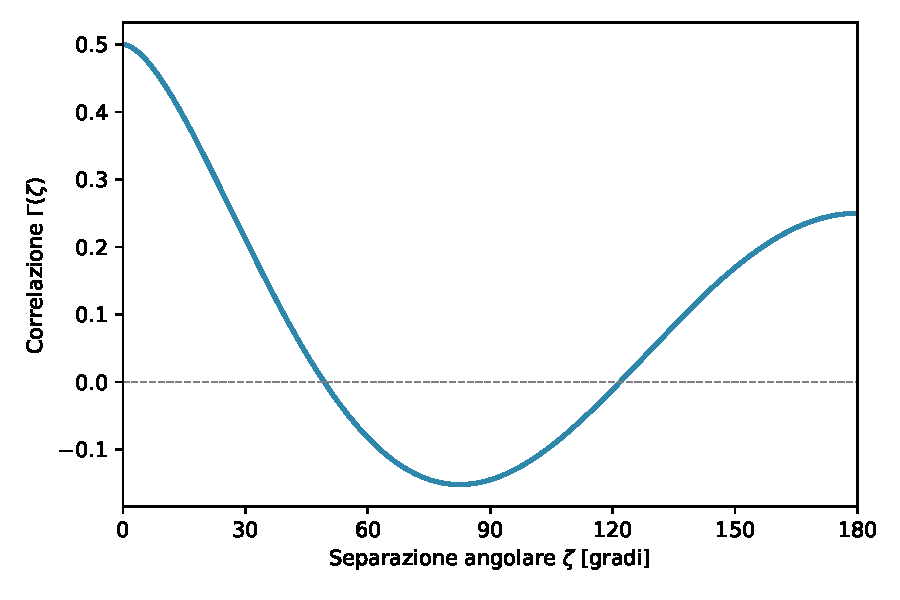
\includegraphics[width=0.7\textwidth]{Figure/cap2/hellings_downs.pdf}
    \caption{\footnotesize Correlazione di Hellings e Downs [Eq.~\eqref{eq:HD}] tra i residui di due pulsar in funzione della loro separazione angolare $\zeta$, per un fondo di onde gravitazionali isotropo e non polarizzato.}
    \label{fig:HD}
\end{figure}

Per il segnale nella singola pulsar (la ``autocorrelazione'') conta invece solo lo spettro: mediando la risposta~\eqref{eq:redshift_GW} sulle direzioni di provenienza e passando dal redshift al residuo tramite la~\eqref{eq:residuo_GW}, che in frequenza corrisponde a dividere per $(2\pi f)^2$ lo spettro di potenza, si ottiene esattamente la densità spettrale~\eqref{eq:psd_gwb}, $S_{\mathrm{GWB}}(f) = h_c^2/(12\pi^2 f^3)$~\cite{Taylor2021}. È questa la componente del GWB che compare nell'analisi di una singola pulsar come quella svolta in questa tesi.

%%%%%%%%%%%%%%%%%%%%%%%%%%%%%%%%%%%%%%%%%%%%%%%%%%%%%%%%%%%%%%%%%%%%%%%%%%%%%%%%%%%%%%%%%%
\section{I Pulsar Timing Array oggi} \label{sec:PTA_oggi}

Esistono diverse collaborazioni PTA nel mondo: l'europea EPTA, che collabora con l'indiana InPTA; la nordamericana NANOGrav; l'australiana PPTA; la cinese CPTA e, più recentemente, MeerKAT PTA in Sudafrica. Dati e analisi vengono condivisi nell'ambito dell'\textit{International Pulsar Timing Array} (IPTA)~\cite{Shaifullah2025}.

Nel giugno 2023 diverse collaborazioni hanno pubblicato in modo coordinato i risultati delle proprie analisi~\cite{EPTA2023_GWB, NANOGrav2023, PPTA2023, CPTA2023}. Tutte hanno trovato un processo rosso comune a tutte le pulsar, con ampiezza di qualche $10^{-15}$ per $\gammagwb = 13/3$, compatibile con le previsioni per una popolazione di SMBHB, e indicazioni della correlazione di Hellings e Downs con una significatività che varia da un dataset all'altro, nei casi migliori di circa $3$--$4\sigma$. % TODO: controllare i numeri esatti nei singoli paper
Per l'EPTA DR2, che comprende 25 MSP osservate da sei radiotelescopi europei su un arco temporale fino a circa 25 anni, l'evidenza più forte emerge nel sottoinsieme dei dati più recenti, acquisiti con strumentazione di nuova generazione (\textit{DR2new}); lasciando libero l'indice spettrale, l'analisi di questo sottoinsieme favorisce $\log_{10}\Agwb \simeq -14$ e $\gammagwb \simeq 2.7$~\cite{EPTA2023_GWB}. % TODO: verificare valori (log10A = -13.94, gamma = 2.71?)

Non si tratta ancora di una rivelazione definitiva, convenzionalmente associata a una significatività di $5\sigma$, e l'interpretazione astrofisica del segnale (incluso il valore di $\gammagwb$, che sembra preferire valori inferiori a $13/3$) è ancora oggetto di studio. Un ruolo centrale in questo dibattito è giocato dalla modellizzazione del rumore delle singole pulsar~\cite{EPTA2023_noise, Ferranti2025}: poiché il segnale gravitazionale e diverse componenti di rumore hanno la stessa forma spettrale a legge di potenza, una descrizione inadeguata del rumore può assorbire parte del segnale o, al contrario, simularlo. Le possibili \textit{degenerazioni} tra i parametri del modello di rumore di una pulsar, e tra questi e un eventuale GWB, sono l'oggetto di questa tesi.
